\documentclass[12pt]{article}
\usepackage{geometry}
\geometry{letterpaper, left=22.5mm, right=22.5mm, top=30mm, bottom=30mm}
\geometry{letterpaper}
\usepackage{amsmath}
\usepackage{amssymb}
\usepackage{enumitem}
\usepackage{fancyhdr}
\usepackage{framed}
\usepackage{tikz}
\usepackage{mathpazo}
%\usepackage{charter}
%\usepackage{newcent}
\usepackage{indentfirst}
\usepackage{booktabs}
\usepackage{graphicx}
\usepackage{float}
\usepackage{makecell}
\usepackage{xcolor}
\usepackage{mdframed}
\usetikzlibrary{trees}
\pagestyle{fancy}
\usepackage{amsthm}
\theoremstyle{definition}
\newtheorem{definition}{Definition}[section]
\theoremstyle{property}
\newtheorem{property}{Property}[section]
\theoremstyle{assumption}
\newtheorem{assumption}{Assumption}[section]
\theoremstyle{example}
\newtheorem{example}{Example}[section]
\theoremstyle{comment}
\newtheorem{comment}{Comment}[section]
\newtheorem{theorem}{Theorem}[section]
\newtheorem{corollary}{Corollary}[theorem]
\newtheorem{lemma}[theorem]{Lemma}
\usepackage{lastpage}
\usepackage{wrapfig}
\usepackage{hyperref}
\usepackage{subcaption}
\usepackage{setspace}
\hypersetup{
colorlinks=true,
filecolor=green, 
urlcolor=blue,
}
\newcommand{\ROM}[1]
    {\MakeUppercase{\romannumeral #1}}
\fancyhead[L]{Econometrics \ROM{2}: Recitation 12 }%change each reci
\fancyhead[R]{Spring 2020}
\fancyfoot[C]{\thepage \hspace{1pt} / \pageref*{LastPage}}

\fancypagestyle{firstpage}{%
\fancyhf{}%
\renewcommand{\headrulewidth}{0mm}%
  \fancyfoot[C]{\thepage \hspace{1pt} / \pageref*{LastPage}}
}

\lhead{Introduction to Econometrics}

\rhead{Recitation 7}


\title{Introduction to Econometrics: Recitation 8}

\begin{document}
\linespread{1.25}
\author{Seung-hun Lee}
\date{November 29th, 2021 }
\maketitle
\section{Instrumental Variable Regression}
\subsection{Motivation}
Recall that when there is a possibility of three of the internal validity threat factors - namely omitted variable bias, measurement error, and simultaneity bias - then we run into the case where the OLS estimation gives us biased estimates. Specifically, these cases bias our result because the error term $u$ is no longer expected to be 0 conditional on $X$ ($E[u|x]\neq 0$). \par\medskip

This is where \textbf{instrumental variables regression} comes in handy. Instrumental variables allow us to eliminate bias in the following sense: When you have an independent variable $X$, there are parts of this variable that are correlated with $u$ and the other parts that are independent of $u$. If we are able to find $Z$ that is correlated with $X$ but not with $u$, using this $Z$ variable would allow you to sort variable $X$ into what is correlate with $u$ and what is not. Then, using the part that is not correlated with $u$, variable $Z$ allows us to get unbiased estimates. \par\medskip

This approach can be very useful in so many settings. Most of our independent variables are \textbf{endogenous} in the sense that $X$ is not a given, but determined as a result of \textit{choice} of individuals, along with dependent variable $Y$. For instance, If $Y$ variable is test score and $X$ is time spent studying, it is possible that the estimates of the effect of time spent studying can be biased. Think about the case where you see your friend (or rival, whichever you prefer) get a really high score. After you know that this person spends a lot of time studying, you decide to study more. Effectively, you see your friend's $Y$ and that affects your selection of $X$ - simultaneity bias. Alternatively, there might be factors uncontrolled by this regression affecting your choice of study hours  - maybe hours spent commuting to schools. Lastly, the measure of $X$ might be inaccurate - for instance, there might be a case where you think you are studying but in reality, it is not. These cases can be addressed by finding some variables that are related with time spent studying but is not correlated with the error term. 

\subsection{IV conditions}
Unfortunately, not every IV is found easily (in fact, you might be able to rebut my examples above). Finding variables that qualify as IV is challenging. The conditions they should satisfy are
\begin{description}
\item[\textbf{Relevance}]: Variable $Z$ satisfies relevancy condition if $cov(X,Z)\neq0$
\item[\textbf{Exogeneity}]: Variable $Z$ satisfies exogeneity condition if $cov(Z,u)=0$
\end{description}
In words, variable $Z$ should be somewhat correlated with the original independent variable $X$. Additionally, variable $Z$ should not be correlated with $u$. The last part seems a bit challenging to conceptualize. So I will introduce another way of thinking about this condition.
\begin{description}
\item[\textbf{Exclusion}]: Variable $Z$ satisfies exclusion condition if it affects $Y$ only through $X$. In other words, when $X$ is controlled for, $Z$ alone should not affect $Y$.
\end{description}
So how does this condition come in? Suppose that your model is (I skip subscript $i$ for convenience) $Y=\beta_0+\beta_1X+u$. Then $cov(Z,u)=0$ can be re-written as
\[
\begin{aligned}
cov(Z,u)&=cov(Z,Y-\beta_0-\beta_1X)\\
&=cov(Z,Y)-cov(Z,\beta_0)-cov(Z,\beta_1X)\\
\end{aligned}
\]
By imposing $cov(Z,u)=0$ and the fact that the covariance of a random variable with a fixed constant is 0, I can get that
\[
cov(Z,Y)=cov(Z,\beta_1X)
\]
This condition means that Z is correlated with Y \textit{only through X}. If there is something else other than $cov(Z,\beta_1X)$ in the right hand side, then this is a violation of the exclusion condition because there is a covariance between $Z$ and $Y$ that is not explained by $X$. If this happens, the IV estimation fails to be accurate. 

\subsection{IV estimation}
There are many ways to estimate IV. I will be introducing \textbf{Two stage least squares}, \textbf{covariance method}, and \textbf{derivations from the reduced form}. 


\subsubsection{Two stage least squares} % mention that first stage standard error
From the disussion in the beginning, IV estimation allows us to separate $X$ into the part that is correlated with $u$ and uncorrelated with $u$. This methods explicitly shows how that is done. The steps for carrying out this approach is as follows:
\begin{enumerate}
\item \textbf{Regress with $X$ as dependent, $Z$ as independent variable.} You will get an equation that looks like
\[
X=\delta_0 + \delta_1Z+v
\]
From this regression, obtain the predicted values of $X$, denoted as $\hat{X}=\hat{\delta}_0+\hat{\delta}_1Z$. This $\hat{X}$ is the part that is related with $Z$ but is uncorrelated with $u$.
\item \textbf{Regress with $Y$ as dependent, $\hat{X}$ as independent variable.} Regressing with this $\hat{X}$ will satisfy the $E[u|\hat{X}]=0$ condition, as the $\hat{X}$ is uncorrelated with $u$, as obtained in the previous step. Thus, your regression equation looks like this:
\[
Y=\beta_0+\beta_1\hat{X}+u
\]
Then you run a OLS regression on the above equation and get the two stage least squares estimator $\hat{\beta}_{\text{TSLS}}$. 
\end{enumerate} \par\medskip
There is one caveat to this method. In particular, you should be careful about what standard errors you are using. If you take the second stage standard error as is, then you end up with wrong standard errors. This is because the second stage standard error does not take into account that you obtained $\hat{X}$ using a separate (first stage) regression. The following example should make things clear. Going back to the regression on cigarette demand in 1995, we are interested in how demand for cigarettes is affected by income and price of cigarettes. In other words,
\[
\ln{Q_i^d}=\beta_0+\beta_1\ln{P_i^d}+u_i
\]
Because quantity demanded can affect price of cigarettes, there is a simultaneity bias. To get around this, we use general sales tax per pack. The following figures demonstrate two different standard errors.
\begin{figure}[H]
\centering
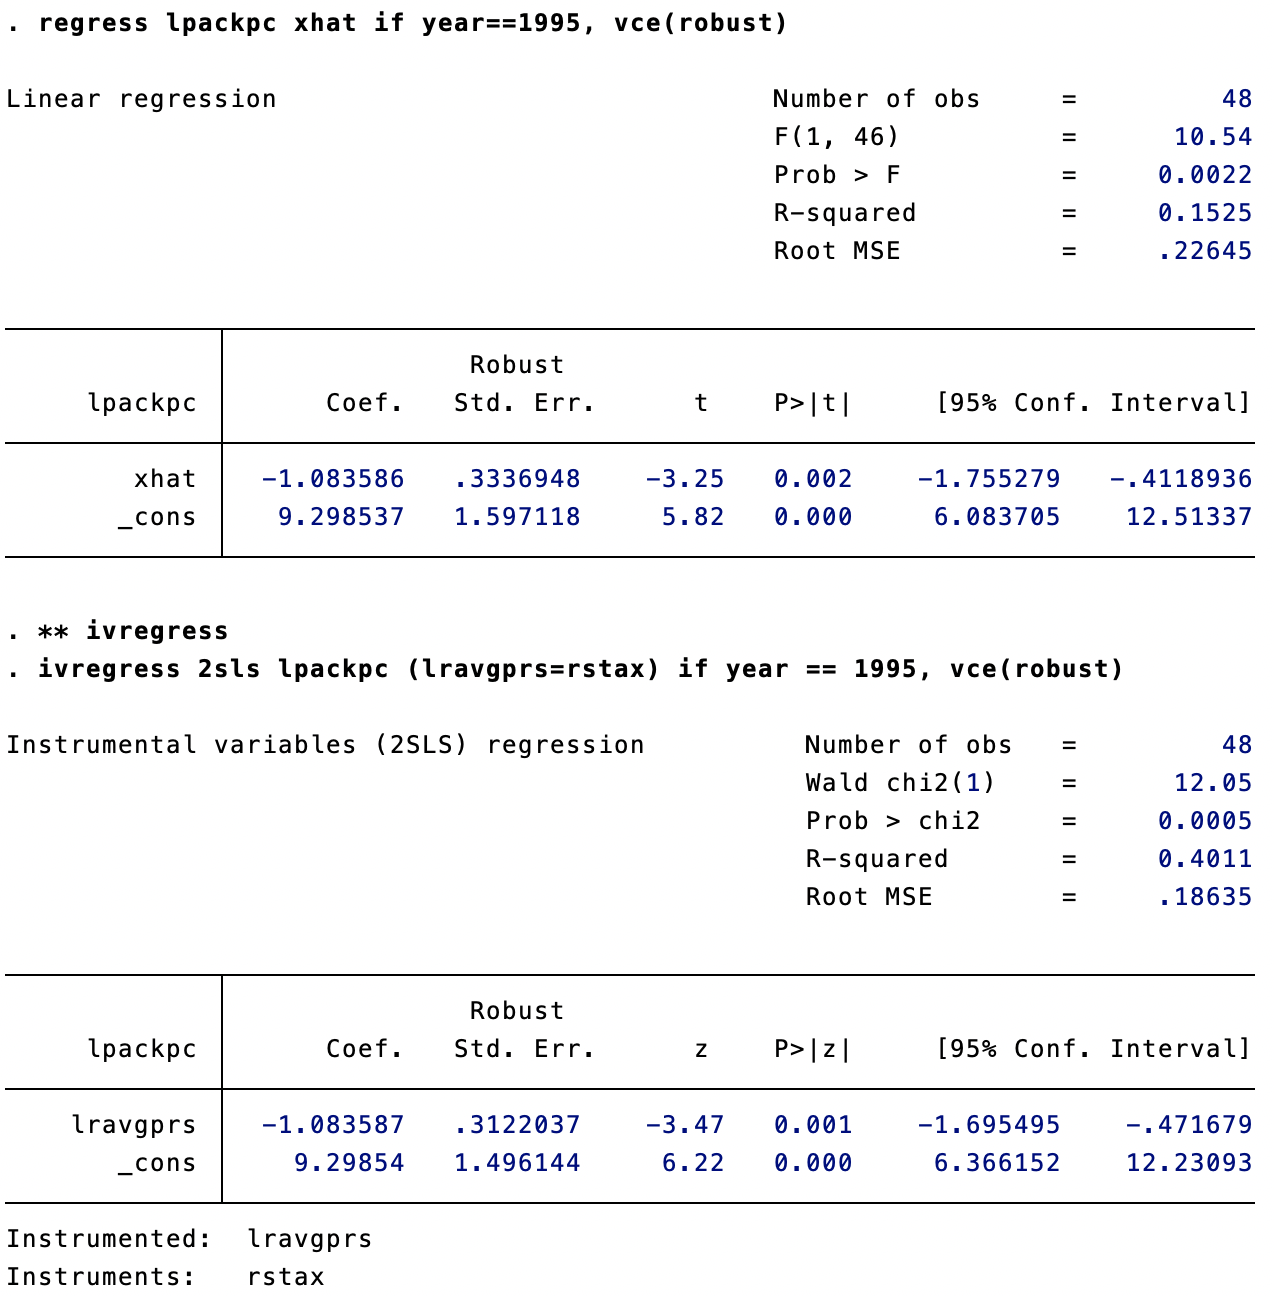
\includegraphics[width=0.5\textwidth,keepaspectratio]{ivregress.png}
\end{figure}
Notice that the standard errors are different. Therefore, if you want to work with correct standard errors, you must use \texttt{ivregress 2sls y x1 (x2 = z)} command.
\subsubsection{Covariance method}
Go back to the part where we discussed the exclusion condition. From there, get
\[
cov(Z,Y)=cov(Z,\beta_1X) \implies cov(Z,Y)=\beta_1cov(Z,X)
\]
From this, we can get
\[
\beta_1=\frac{cov(Z,Y)}{cov(Z,X)}
\]
where division is possible because we require a relevancy condition ($cov(Z,X)\neq0$). If you replace the population covariances with sample covariances, we get the IV estimator
\[
\hat{\beta}_{TSLS}=\frac{s_{ZY}}{s_{ZX}}
\]
\subsubsection{Derivations from the reduced form}
This requires some amount of algebra. Denote the two equations as
\begin{gather*}
X=\pi_0+\pi_1Z+v \ (\text{where }cov(Z,v)=0)\\ Y=\gamma_0+\gamma_1Z+w \ (\text{where }cov(Z,w)=0)
\end{gather*}
When you rewrite the first equation in terms of $Z$, you get
\[
Z=\frac{X}{\pi_1}-\frac{\pi_0}{\pi_1}-\frac{v}{\pi_1}
\]
Then plug this into the second equation. Reorganizing this equation, you should get
\[
Y=\left(\gamma_0-\frac{\pi_0\gamma_1}{\pi_1}\right)+\left(\frac{\gamma_1}{\pi_1}\right)X+\left(w-\frac{\gamma_1}{\pi_1}u\right)
\]
What this gets you is that $\beta_1$ from the equation where we had $X$ as independent variable is $\beta_1 = \frac{\gamma_1}{\pi_1}$. This also implies that when $Z$ rises by 1 unit, $X$ exogenously changes by $\pi_1$ units and $Y$ changes by $\gamma_1$ as a result. In other words, 1 unit of exogenous change in $X$ translates to  $\beta_1 = \frac{\gamma_1}{\pi_1}$ units of change in $Y$. \par\medskip



\subsection{Properties of IV estimators}
Note that the IV estimator can be written in terms of the ratios of the two covariances. In sample analogs, it is written as
\[
\hat{\beta}_{1,\text{TSLS}}=\frac{s_{zy}}{s_{zx}}\simeq\frac{\frac{1}{n}\sum_{i=1}^n(Z_i-\bar{Z})(Y_i-\bar{Y})}{\frac{1}{n}\sum_{i=1}^n(Z_i-\bar{Z})(X_i-\bar{X})}
\]
Note that $\frac{1}{n}\sum_{i=1}^n(Z_i-\bar{Z})(Y_i-\bar{Y})$ is not an unbiased estimator for the covariance of $Z,Y$ (and similar for $\frac{1}{n}\sum_{i=1}^n(Z_i-\bar{Z})(X_i-\bar{X})$) If you have large samples, however, then $\frac{1}{n}\sum_{i=1}^n(Z_i-\bar{Z})(Y_i-\bar{Y}$) is a \textbf{consistent} for covariance of $Z,Y$\footnote{However, $\frac{1}{n-1}\sum_{i=1}^n(Z_i-\bar{Z})(Y_i-\bar{Y})$ is unbiased. For more information refer to \url{https://math.stackexchange.com/questions/2019122/unbiased-estimate-of-the-covariance}}. In mathematical terms, $s_{YZ}\xrightarrow{p} cov(Y,Z),  s_{XZ}\xrightarrow{p} cov(X,Z)$. With these properties, we can say that the IV estimator of $\beta_1$, which is $\hat{\beta}_{1,\text{TSLS}}$ is a consistent estimator for the true $\beta_1$ \par\medskip

The notion of IV estimation does not change much even in multiple regression settings. Suppose that we have
\[
Y_i = \beta_0 + \beta_1X_{1i} +...+ \beta_kX_{ki} + \delta_1W_{1i}+...+\delta_lW_{li}+u_i 
\]
where $X$ variables are endogenous and $W$ variables are exogenous. Assume that we have found a total of $m$ (not necessarily, equal. We'll save the discussion to overidentification test) variables that could qualify as IVs. Additionally, IV regression requires these assumptions 
\begin{description}
\item[\textbf{IV1}] $E[u_i|W_{1i},...,W_{li}]=0$ (At least for exogenous variables, this is satisfied)
\item[\textbf{IV2}] $(Y_i,X_{1i},..,X_{ki},W_{1i},..,W_{li},Z_{1i},...,Z_{mi})$ are IID
\item[\textbf{IV3}] The $Y,X,W,Z$ variables all have nonzero finite 4th moments
\item[\textbf{IV4}] The instruments are valid. That is $cov(Z_{ji},u_i)=0$ for all $j=1,...,m$ and relevancy conditions are satisfied for all $Z$'s. 
\end{description}
\subsection{Identification issues}
In a general sense, a parameter is \textbf{identified} if different values of the parameter produce different distributions of the data. In other words, there is a one-to-one matching of the parameters and the distributions. For instance, A normal distribution with mean $\mu$ and variance $\sigma^2$ is identified because different values of $\mu, \sigma^2$ produce different distributions. If it is the case that the same distribution can be obtained from different parameter values, we say that the parameters are not identified. \par\medskip

In the context of IV's, the parameters we are interested are coefficients for the independent variables. This depends on how much instrument variables ($m$ in the previous section) we have relative to the endogenous variables ($k$). There are three possible cases
\begin{description}
\item[\textbf{Just-identified}]: When $m=k$. There are just enough instruments to identify $k$ endogenous variables
\item[\textbf{Overidentified}] When $m>k$. There are more than enough instruments. We later test whether the instruments are valid using \textbf{overidentification test}.
\item[\textbf{Underidentified}] When $m<k$. There are not enough instruments. The coefficients for $X$'s will not be identified 
\end{description}
So the key takeaway here so far is that when you are using IV, you need at least as much instrumental variables as the number of endogenous regressors you have. Now the issue is having too much IV bad? That depends on the answer we get from the overidentification test, which we cover in the next section.\par\medskip

\subsection{Implementing tests to verify that IV conditions hold}
\subsubsection{Underlying distribution of the IV estimators}
As with other estimators, we need to understand the the distribution of IV estimators in order to conduct any sort of tests. Fortunately, IV estimators, at least in the large numbers, have normal distribution. This means there is no drastic changes in the critical values and confidence intervals we select when we conduct hypothesis tests. So why is that the case? We can find this out by breaking down the 2SLS estimator into the following
\[
\begin{aligned}
\hat{\beta}_{\text{TSLS}}=\frac{s_{zy}}{s_{zx}}&=\frac{\sum_{i=1}^n(Z_i-\bar{Z})(Y_i-\bar{Y})}{\sum_{i=1}^n(Z_i-\bar{Z})(X_i-\bar{X})}\\
&= \frac{\sum_{i=1}^n(Z_i-\bar{Z})Y_i}{\sum_{i=1}^n(Z_i-\bar{Z})X_i}\\
&= \frac{\sum_{i=1}^n(Z_i-\bar{Z})(\beta_0+\beta_1X_i + u_i)}{\sum_{i=1}^n(Z_i-\bar{Z})X_i}\\
&= \beta_1+\frac{\sum_{i=1}^n(Z_i-\bar{Z})u_i}{\sum_{i=1}^n(Z_i-\bar{Z})X_i}=\beta_1+\frac{\frac{1}{n}\sum_{i=1}^n(Z_i-\bar{Z})u_i}{\frac{1}{n}\sum_{i=1}^n(Z_i-\bar{Z})X_i}\\
\end{aligned}
\]
After subtracting both sdies by $\beta_1$ and multiplying both sides by $\sqrt{n}$, we get
\[
\sqrt{n}(\hat{\beta}_{\text{TSLS}}-\beta_1)=\frac{\frac{1}{\sqrt{n}}\sum_{i=1}^n(Z_i-\bar{Z})u_i}{\frac{1}{n}\sum_{i=1}^n(Z_i-\bar{Z})X_i}
\]
Note that the denominator converges to $cov(Z,X)$ by (weak) law of large numbers and the numerators converges to $N(0, var[(Z-\mu_Z)u])$ by central limit theorem. Thus, $\hat{\beta}_{\text{TSLS}}$ has a normal distribution.
\subsubsection{Confirming relevance of the instruments}
We introduce a test to confirm that the instruments are really relevant. Assume we have
\[
Y_i = \beta_0 + \beta_1X_i + \beta_2 W_{1i}+...+\beta_{1+r}W_{ri}+u_i
\]
where only $X_i$ is endogenous. Suppose we have $m$ instruments. Then our first stage equation looks like
\[
X_i = \pi_0 + \pi_1Z_{1i}+...+\pi_mZ_{mi} + \pi_{(m+1)i} W_{1i}+...+ \pi_{(m+r)i}W_{ri}+v_i
\]
We say our instrument is relevant if at least one of $\pi_1,...,\pi_m$ is statistically nonzero. To confirm that this is the case, we run the $F$-test with these null and alternative hypothesis
\[
H_0: \pi_1 = ... = \pi_m=0 \ \text{vs.} \ H_1: \lnot H_0
\]
We calculate the $F$-statistics from this test. By rule of thumb, we want to have an $F$-statistics larger than 10. If otherwise, all these coefficients are zero or very close to it. In such case, we have a \textbf{weak instrument} problem - our choice of instruments does little to explain variation in $X_i$.  This affects our inference as the IV estimator may not have a normal distribution even with large numbers of observations. 
\subsubsection{Tests for exogeneity of the instruments}
Here, we partially check for exogeneity of our instruments. Recall that instruments are exogenous if all of them are uncorrelated with the error term. This is how we pick up the part of $X$ that is uncorrelated with $u$ (the $\widehat{X}$). If otherwise, we cannot pick up this part of $X$. We can \textit{partially} test for this (more on this later) when we have more instrumental variables than the endogenous variables ($m>k$ from above section). We call this the test of overidentifying restrictions.
\par
Consider the following case: We want to regress
\[
Y_i = \beta_0 + \beta_1X_{1i} +...+ \beta_kX_{ki} + \delta_1W_{1i}+...+\delta_lW_{li}+u_i 
\]
and we found $m$ possible candidates for instrumental variables, $Z_1,...,Z_m$. Overidentifying restriction test we conduct here is a $J$-test that uses TSLS estimators and not the hypothesized $\beta$ values. The steps are as follows
\begin{enumerate}
\item Regress the above equation using 2SLS.
\item Obtain the residuals $\hat{u}_i=Y_i-\widehat{Y}_i$
\item Regress residuals onto instruments and other controls, namely
\[
\hat{u}_i = \alpha_0 + \alpha_1 Z_{1i}+ ... + \alpha_m Z_{mi} + \alpha_{m+1}W_{1i}+ ... + \alpha_{m+l}W_{li}+v_i
\]
\item Compute the $F$-statistics from the following hypothesis
\[
H_0: \alpha_1 = ... = \alpha_m=0\ \text{vs.} \ H_1: \lnot H_0
\]
\item Derive the $J$ statistics as follows $J = m\times F$. $J$ follows $\chi^2_{m-k}$ distribution 
\item If there are endogenous instruments, the $\alpha$ coefficient for that instrument will not be 0. This will inflate the $J$ statistic to the extent that you reject the null of exogenous instruments. (Note that rejecting the null in this case is not something that you want!)
\item If the test is rejected, you need to make a guess on which instrument is violating the exogeneity condition, drop those, and redo the above procedure. (Good luck!)
\end{enumerate}
There are some other ways to understand this. Suppose that we only have one independent variable that is also endogenous  -$X_i$. Also suppose that we have two instrumental variables - $Z_{1i}, Z_{2i}$. Now, we run two two-stage least squares regression with each one of the instrumental variables. The estimates for the coefficient for $X$ are 
\[
\hat{\beta}_{Z_1}=\frac{cov(Z_1,Y)}{cov(Z_1,X)}, \ \hat{\beta}_{Z_2}=\frac{cov(Z_2,Y)}{cov(Z_2,X)}
\]
The numbers look different, although both $\hat{\beta}$'s are suppose to be the same coefficient estimating impact of $X_1$ on $Y$. The overidentification test checks whether the differences between $\hat{\beta}_{Z_1}, \hat{\beta}_{Z_2}$ are large. If the two estimates are similar in the sense that the sample analogs of both $\frac{cov(Z_1,Y)}{cov(Z_1,X)}$ and $\frac{cov(Z_2,Y)}{cov(Z_2,X)}$ converge to the same thing in probability, we don't really have to worry. If they converge to something different, then we may have problem with either one or potentially both instrumental variables. Therefore, the takeaway from overidentification test is that it checks whether there exists a faulty IV variable in the case where we found too many candidates for instrumental variables. 
\par
So what do we do in just identified case? To be very honest, there is not much we can do in terms of rigorous testing approach. This is usually the area of judgement call. One way to do this is to use the approach of exclusion restriction - you argue that the instrumental variable $Z$ affects $Y$ only through $X$. If $Z$ affects $Y$ directly without $X$, then the exclusion restriction fails. You try to persuade others based on logic, previous practices, or intuition (usually a combination of all three). This is what I meant in the beginning when I said we can partially test for exogeneity conditions. 
%%%%%%%%%%%%%%%%
\end{document}

